\section{Liouville equation and the pendulum}

Consider the pendulum of length l and mass m in a gravitational field
g. The kinetic energy and potential energy are
\begin{equation}
    T=\frac{1}{2}ml^2\dot{\theta}^2
\end{equation}
and 
\begin{equation}
    V=mgl(1-\cos\theta)
\end{equation}

\subsection{}
%Derive the Hamiltonian and write down Hamilton’s equations.
Starting from the Lagrangian, 
\begin{equation*}
    \mathcal{L}(\theta,\dot{\theta},t)\equiv T-V = \frac{1}{2}ml^2\dot{\theta}^2 - mgl(1 - \cos\theta),
\end{equation*}
we can find the generalized momentum by
\begin{align*}
    p\equiv\frac{\partial\mathcal{L}}{\partial\dot{q}}=ml^2\dot{\theta}.
\end{align*}
Then the Hamiltonian is
\begin{align*}
    \mathcal{H}&\equiv T+V\\
    \mathcal{H}&=\frac{1}{2}ml^2\dot{\theta}^2+mgl(1-\cos\theta)\\
    \mathcal{H}&=\frac{1}{2}\frac{p^2}{ml^2}+mgl(1-\cos\theta).
\end{align*}

Hamilton's equations are:
\begin{align*}
    \dot{p}&\equiv-\frac{\partial\mathcal{H}}{\partial\theta}=-mgl\sin\theta\\
    \dot{q}&\equiv\frac{\partial\mathcal{H}}{\partial p}=\frac{p}{ml^2}=\dot{\theta}
\end{align*}

\subsection{}
%Transform these equations to a non-dimensional set of variables $(q,p)\to(z_1,z_2)$ such that $\tau=\omega t$ where $\omega^2=g/l$ and the dimensionless energy is:
% \begin{equation}
%     \varepsilon\equiv\frac{E}{mgl}=\frac{1}{2}z_2^2+(1-\cos z_1)
% \end{equation}
% Show that $\tau_0=2\pi/\omega$ is the period of small oscillations  for this system.
From the dimensionless energy $\varepsilon=E/mgl$ 
\begin{align*}
    \varepsilon&=\frac{1}{mgl}\left[\frac{1}{2}ml^2\dot{\theta}^2+mgl(1-\cos\theta)\right]\\
    &=\frac{1}{2}\frac{l}{g}\dot{\theta} + (1-\cos\theta),
\end{align*}
we can find the dimensionless variables as
\begin{align*}
    z_1\equiv\theta\\
    z_2\equiv\frac{l}{g}\dot{\theta}=\frac{\dot{\theta}}{\omega^2}
\end{align*}
where $\omega^2=g/l$.

Knowing that the equation of motion for this system is 
\begin{equation*}
    \Ddot{\theta}=-\frac{g}{l}\sin\theta
    \label{eq:pendEqMotion}
\end{equation*}
we can find that the solution for this differential equation in the small angle approximation will be given by
\begin{equation*}
\frac{dz_2}{d\tau}=\frac{d}{dt}
\frac{\Ddot{\theta}}{\omega^2}=    
\end{equation*}

then, we can show that
$\tau_0=2\pi/\omega$.

\subsection{}
%Sketch the phase portrait in these units, paying special attention to
% the three domains: 1) $\varepsilon<2$, the oscillation  or libration regime; 2) $\varepsilon>2$, the rotation regime 3)$\varepsilon=2$, the critical infinite period, the separatrix.

\begin{figure}[h]
    \centering
    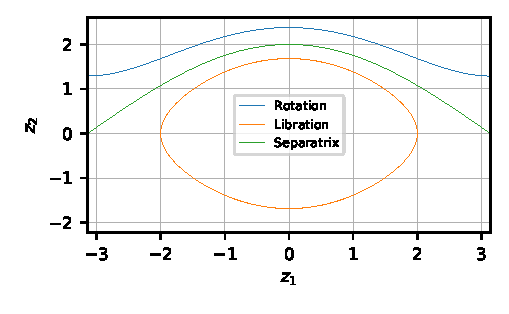
\includegraphics{CodeAndFigures/PendulumPhaseSpace.pdf}
    \caption{Phase Space of a pendulum in rotation ($\varepsilon>2$), libration ($\varepsilon<2$) and separatrix ($\varepsilon=2$).}
    \label{fig:pendPhaseSpace}
\end{figure}

We can integrate the pendulum's equation of motion \ref{eq:pendEqMotion} using a 4th order Runge-Kutta and the initial conditions listed in table \ref{tab:pendulumIV}.

\begin{table}[h]
    \centering
    \begin{tabular}{lrrr}
\toprule
{} &  $z_1$ &  $z_2$ &  Energy \\
\midrule
Rotation   &  -4.71 &   1.91 &    2.83 \\
Libration  &  -1.57 &   0.91 &    1.42 \\
Separatrix &  -4.71 &   1.41 &    2.00 \\
\bottomrule
\end{tabular}

    \caption{Initial conditions used for obtaining the phase-space of the pendulum for rotation, libration and separatrix.}
    \label{tab:pendulumIV}
\end{table}

Figure \ref{fig:pendPhaseSpace} shows the phase space in the three domains: rotation, libration and separatrix.

\subsection{}
Considering a disk-like of initial conditions enclosed within a circle centered at $(q,p)=(z_1,z_2)=(0,1)$ with radius of $1/2$ as shown in Figure \ref{fig:MartinsUs}, we can compute the evolution of the disk from $\tau=0$ to each of $\tau=0.25\tau_0,0.5\tau_0,\mathrm{and}\tau_0$.
\begin{figure}[h]
    \centering
    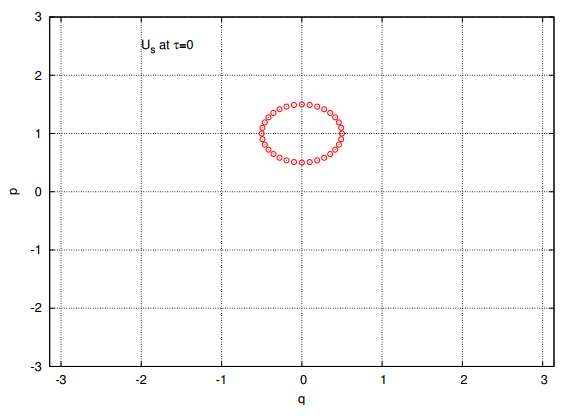
\includegraphics[width=\columnwidth]{CodeAndFigures/Fig1InitialConditionsUs.png}
    \caption{Initial conditions for $U_s$}
    \label{fig:MartinsUs}
\end{figure}

Figure \ref{fig:pend2d} shows the evolution of 32 orbits equally spaced at different times obtained from 4th order Runge-Kutta integration. The color disks shows the final values of $(z_1,z_2)$ at the different stop times as shown. Note that the orbits are parallel through time and don't cross each other so we can argue that calculating the orbits at the edge of the disk put a constraint on orbits at any point inside the disk. Additionally we can confirm that all of these orbit are in the libration regime since the go around in a circle and seem to reach the same spot.

%Consider a disk-like domain of initial configurations $U_s$ enclosed
% within the circle centered at $(q,p)=(z_1,z_2)=(0,1)$ with radius
% of $1/2$ in these units. See Fig. 1 for a plot of these initial conditions. Compute the evolution of the disk from $\tau=0$ to each of $\tau=0.25\tau_0,0.5\tau_0,\mathrm{and}\tau_0$.
% Remarks:
%     \begin{itemize}
%     \item Argue that it is sufficient to compute the
%           trajectories on the
%           circle at edge of the disk. In other words, a point
%           on the inside of the disk can not pass through
%           a boundary point.
%     \item You may solve this any way you like. E.g. there is 
%           an analytic solution in terms of elliptic 
%           integrals. But I recommend an numerical solution, 
%           using your RK4 routine to solve the equations of
%           motion for say 32 points equally spaced around the 
%           circle at the perimeter of $U_s$ at $\tau = 0$.
%     \item For insight consider this problem in the small 
%           angle limit. In this limit, the solution is 
%           analytic. If you have any worries about your 
%           solution, make sure it agrees with the small angle
%           limit.
%     \end{itemize}

\begin{figure}
    \centering
    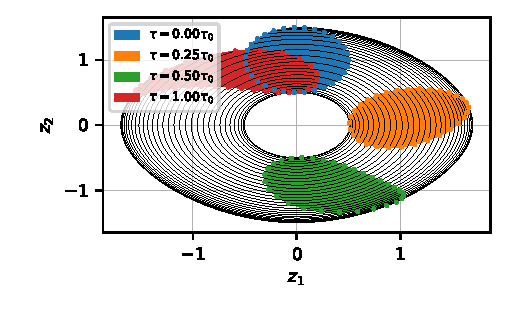
\includegraphics{CodeAndFigures/PendulumPhaseSpaceUs2d.pdf}
    \caption{Evolution of the phase space of 32 orbits using a disk-like shape of initial conditions centered on $(z_1,z_2)=(0,1)$ with a radius of $1/2$.}
    \label{fig:pend2d}
\end{figure}

\subsection{}
% \item Repeat the experiment but now with the circle centered at $(q,p)=(0,1.5)$ Note: some points will be on or near the separatrix. Compute the evolution of the disk for $\tau=0,0.2\tau_0,0.4\tau_0,\mathrm{and}0.75\tau_0$.[NB: the “evolution” at t = 0 is the initial condition, of course.]
\begin{figure}
    \centering
    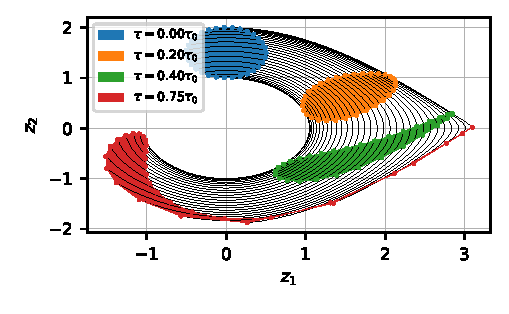
\includegraphics{CodeAndFigures/PendulumPhaseSpaceUs2e.pdf}
    \caption{Evolution of the phase space of 32 orbits using a disk-like shape of initial conditions centered on $(z_1,z_2)=(0,1.5)$ with a radius of $1/2$. }
    \label{fig:pend2e}
\end{figure}

Figure \ref{fig:pend2e} shows the evolution of 32 orbits using the same disk-like shape of initial conditions but now centered on $(z_1,z_2)=(0,1.5)$. As you can note, we continue to have orbits in libration but since we are getting closer to the separatrix the orbits start to have a oblong shape. 

\subsection{}
%Repeat the experiment but now with the circle centered at  $(q,p)=(0,2)$. Compute the evolution at times $\tau=0,0.1\tau_0,0.25\tau_0,\mathrm{and}0.5\tau_0$

\begin{figure}
    \centering
    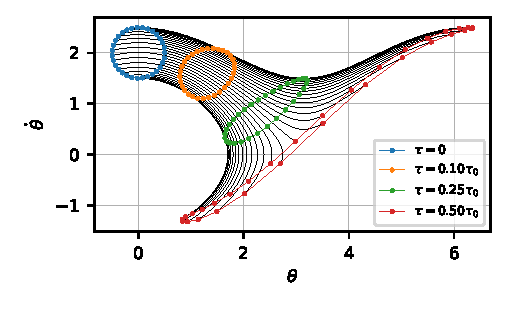
\includegraphics{CodeAndFigures/PendulumPhaseSpaceUs2f.pdf}
    \caption{Evolution of the phase space of 32 orbits using a disk-like shape of initial conditions centered on $(z_1,z_2)=(0,2)$ with a radius of $1/2$.}
    \label{fig:pend2f}
\end{figure}

Figure \ref{fig:pend2f} shows the evolution of 32 orbits but now we centered the disk-like shape of initial conditions on  $(z_1,z_2)=(0,2)$. With this initial conditions we crossed the separatrix and have orbits in rotation.  

\subsection{}
%For each of the three experiment with different disk centers, make
% a plot the disk at each of these times in the $(q,p)$ plane (e.g.
% a phase portrait). Interpret the results. Is Liouville’s theorem obeyed?
We can represent the state of a system of N stars by a point in a 6N-dimensional phase space called $\Gamma$-space and the point described by the coordinates is a $\Gamma$-point.  
Liouville’s theorem states that the flow of $\Gamma$-points through $\Gamma$-space is incompressible. We can calculate the area of our disk-like initial conditions and show that it remains constant through time.

To calculate the area I used the shoelace formula:
\begin{equation}
    A=\frac{1}{2}\sum_{i=1}^N\left(x_{i}y_{i+1}-x_{i+1}y_{i}\right)
\end{equation}
where, for this case, $x=z_1$ and $y=z_2$. 

\begin{figure}
    \centering
    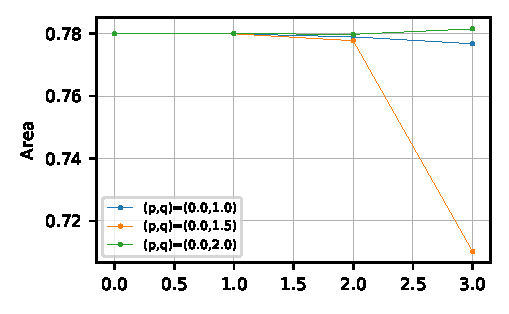
\includegraphics{CodeAndFigures/PendulumPhaseSpaceAreas.pdf}
    \caption{Plot showing the area calculated at the different stop times specified on each corresponding phase space plot.}
    \label{fig:pendAreas}
\end{figure}

Since our disk-like of initial conditions all have a radius of $1/2$ then we can calculate the analytic area to be $\pi r^2 = \pi(.5)^2=0.7854$.

Figure \ref{fig:pendAreas} shows the areas for each set of different initial conditions at the different $\tau$. We can note that they stay constant except for the last time step when the initial conditions are $(z_1,z_2)=(0,1.5)$. I think this is because the disk gets stretch out to the point that the calculated points don't sample the area good enough.
